\documentclass[12pt]{article}
\usepackage{listings}
\usepackage{amsmath}
\usepackage{amssymb}
\usepackage[usenames,dvipsnames]{color}
\usepackage{comment}
\usepackage[T2A]{fontenc}
\usepackage[utf8]{inputenc}
\usepackage[russian]{babel}
\usepackage[parfill]{parskip}
\usepackage{graphicx}
\usepackage{float}
\usepackage{caption}
\usepackage{subcaption}
\usepackage{hyperref}
\everymath{\displaystyle}

\usepackage[margin=1in]{geometry} 
% \oddsidemargin=0.5cm
\definecolor{Orange}{cmyk}{0.0,0.56,0.58,0.11}
\definecolor{Gray}{gray}{0.5}
\lstset{
    language=Java,
    basicstyle=\ttfamily,
    keywordstyle=\color{Orange},
    commentstyle=\color{Gray},
    captionpos=b,
    breaklines=true,
    breakatwhitespace=false,
    showspaces=false,
    showtabs=false,
    numbers=left,
}


\title{Token Ring}
\author{Марина Белялова}
\date{26 ноября 2017}

\begin{document}

\begin{center}


\textsc{\Large Московский Физико-Технический Институт \\ (Государственный университет)}\\[1cm]
\textsc{\normalsize Кафедра банковских информационных технологий}\\[4cm]
{ \huge \bfseries Token Ring \\[1cm] }
\textnormal{\normalsize Выполнила cтудентка 285 гр. Марина Белялова}\\[10cm]
\textnormal{Москва, 2017}
\end{center}

%=============================================================

\newpage

\tableofcontents
%=============================================================

\newpage
\section{Описание задачи}
В данной работе описана реализация модели сетевого протокола Token Ring на языке Java. Целью данной работы являлось исследование зависимости характеристик latency и throughput от числа нод и загруженности нод, а так же поиск варианта оптимизации работы для недогруженного и перегруженного режимов передачи пакетов.

\begin{itemize}
\item Система состоит из $N$ пронумерованных от $0$ до $N-1$ нод. Ноды упорядочены по порядковому номеру. После ноды $N-1$ следует нода $0$, т.е. ноды формируют кольцо. 
\item Соседние в кольце ноды могут обмениваться пакетами. Обмен возможен только по часовой стрелке. 
\item Каждая нода, получив пакет от предыдущего, отдает его следующему.
\item Пакеты не могут обгонять друг друга.
\end{itemize}

\section{Основные сущности и соответствующие классы}
\subsection{Сообщение}
Сообщения, которые передаются в системе, реализованы в классе \lstinline|Message|. Сообщение имеет размер и при отправке фиксирует в себе время. Содержит в себе логическую величину
\lstinline|hasBeenDelivered.|

\subsection{Пакет}
Класс \lstinline|Frame| реализует сущность пакета, который может пребывать в двух состояниях: \lstinline|isToken() = true|, т.е. фрейм пустой и не содержит в себе сообщение, либо фрейм содержит сообщение, которое может быть доставлено или не доставлено. Когда фрейм представляет собой токен, любая нода, желающая отправить сообщение, может использовать этот фрейм.

\subsection{Узел}
Класс \lstinline|Node|, наследник класса \lstinline|Thread|, реализует узел сети. Каждая нода имеет очередь \lstinline|Queue<Message> pendingMessages = new ConcurrentLinkedQueue<>()| сообщений, ожидающих отправки, и очередь входящих фреймов \lstinline|Queue<Frame> enqueuedFrames = new ConcurrentLinkedQueue<>()|. \lstinline|Node| содержит в себе логику обработки входящих фреймов:

\input Classes/Node

В методе \lstinline|void handleIncomingMessage(Frame currentFrame)| успешность доставки сообщения имеет распределение Бернулли с вероятностью успеха $p$. Конкретные значения в экспериментах указаны в соответствующих разделах. В случае успеха нода-получатель ставит метку \lstinline|hasBeenDelivered| у сообщения и записывает в массив \lstinline|List<Double> deliveryTimes| время, затраченное на доставку сообщения. В методе \lstinline|void handleDelivered Message(Frame currentFrame)| нода-отправитель, получая обратно сообщение, прошедшее полный круг и полученное адресатом, высвобождает токен. В методе \lstinline|void handleUndelivered Message(Frame currentFrame)| нода-отправитель реализует логику обработки сообщений, не полученных адресатом, в соответствии с параметром возможного удержания токена token holding time (THT): если время, прошедшее с момента отправки сообщения, превысило THT, то нода удаляет сообщение и выпускает токен. Конкретные значения THT в экспериментах указаны в соответствующих разделах.

\subsection{Генератор сообщений}
Экземпляр класса \lstinline|MessageGenerator|, наследник класса \lstinline|Thread|, помещает сообщение на случайную ноду. События появления сообщений описываются экспоненциальным распределением с характерным временем $\tau=\frac{1}{\lambda}$. Последовательные интервалы времени между появлением сообщений получаются функцией: $F^{-1}(p) = \frac{-ln(1-p)}{\lambda}$, где $p$ – случайная величина, равномерно распределённая в интервале $[0, 1]$. Обоснование выбора того или иного характерного времени приведено в разделе "Основные параметры и метрики".

\subsection{Вспомогательный класс запуска}
Класс \lstinline|Launcher| осуществляет инициализацию нод, фреймов, начальное распределение фреймов по нодам, запуск тредов нод и треда генератора сообщений, остановку тредов по достижении необходимого числа доставленных сообщений, логгирование в файл.

\section{Основные параметры и метрики}
Для измерения времени использовалась системная функция \lstinline|System.nanoTime()|.

Введём следующие параметры запуска:
\begin{itemize}
\item $N$ – число нод.
\item $F$ – число фреймов. 
\item $M$ – целевое число доставленных сообщений. Во всех расчётах было выбрано число $10*N$.
\item $\tau$ – характерное время появления сообщений в генераторе. 
\item THT (token holding time) – время возможного удержания токена.
\end{itemize}

Введём следующие величины, которые рассчитываются по результатам запуска.
\begin{itemize}
\item $T$ – время выполнения.
\item $l$ – среднее время доставки сообщений, т.е. latency. Среднее значений массива \lstinline|List<Double> deliveryTimes|.
\item $t$ – среднее число передаваемых сообщений в единицу времени, т.е. throughput. $t = \frac{M}{T}$.
\item $P$ – среднее число сообщений, передаваемых в системе в единицу времени.
\item $LR$ (load rate) – загрузка системы сообщениями. $LR = \frac{P}{N}$.
\end{itemize}

\subsection{Подбор характерного времени появления сообщений в генераторе $\tau$}
$\tau$ подбиралось таким образом, чтобы обеспечить необходимую загрузку системы сообщениями $P$.
В абстрактной системе, появление новых элементов в которой происходит со средним временем $\tau$, а удаление элементов – со средним временем $l$, среднее число элементов будет составлять $\frac{l}{\tau}$. Однако, в нашей системе есть ограничение числа передаваемых сообщений сверху: число фреймов $F$. Таким образом, 
\begin{gather}
P=min\{\frac{l}{\tau}, F\}
\end{gather}
Чтобы обеспечить $P=F$, будем задавать $\tau < {\frac{l}{F}}$.
Таким образом, далее будем считать, что $P=F$, и исследовать зависимость интересующих нас величин не от $P$, а от $LR= \frac{P}{N}= \frac{F}{N}$.

\subsection{Характеристики процессора}
Вычисления проводились на процессоре Intel Core i5 3337U. 
\begin{figure}[H]
\centering
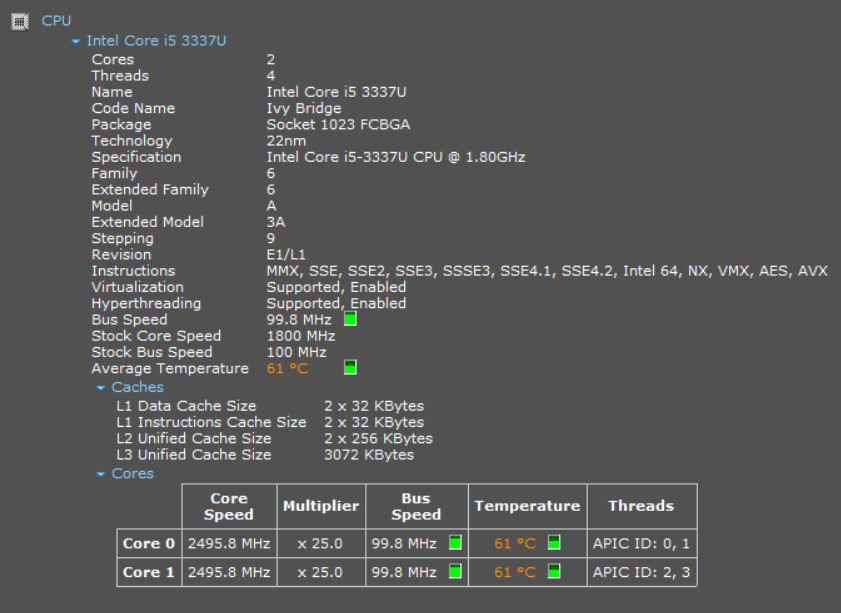
\includegraphics[width=1.0\textwidth]{Plots/intel.png}
\caption{Характеристики процессора}
\end{figure}


\section{Исследование зависимости latency и throughput от числа нод и загруженности нод}

\subsection{Параметры}
Вероятность успеха доставки сообщения $p=0.85$.

THT (token holding time) = \lstinline|Double.MAX_VALUE| (без ограничения сверху на время доставки сообщения).

$N$ принимало значения \lstinline|{5, 10, 15, 25, 50, 65, 85, 100}|. 

$LR$ принимало значения \lstinline|{0.2, 0.4, 0.6, 0.8, 1.0}|.

\subsection{Результаты}
\begin{figure}[H]
\centering
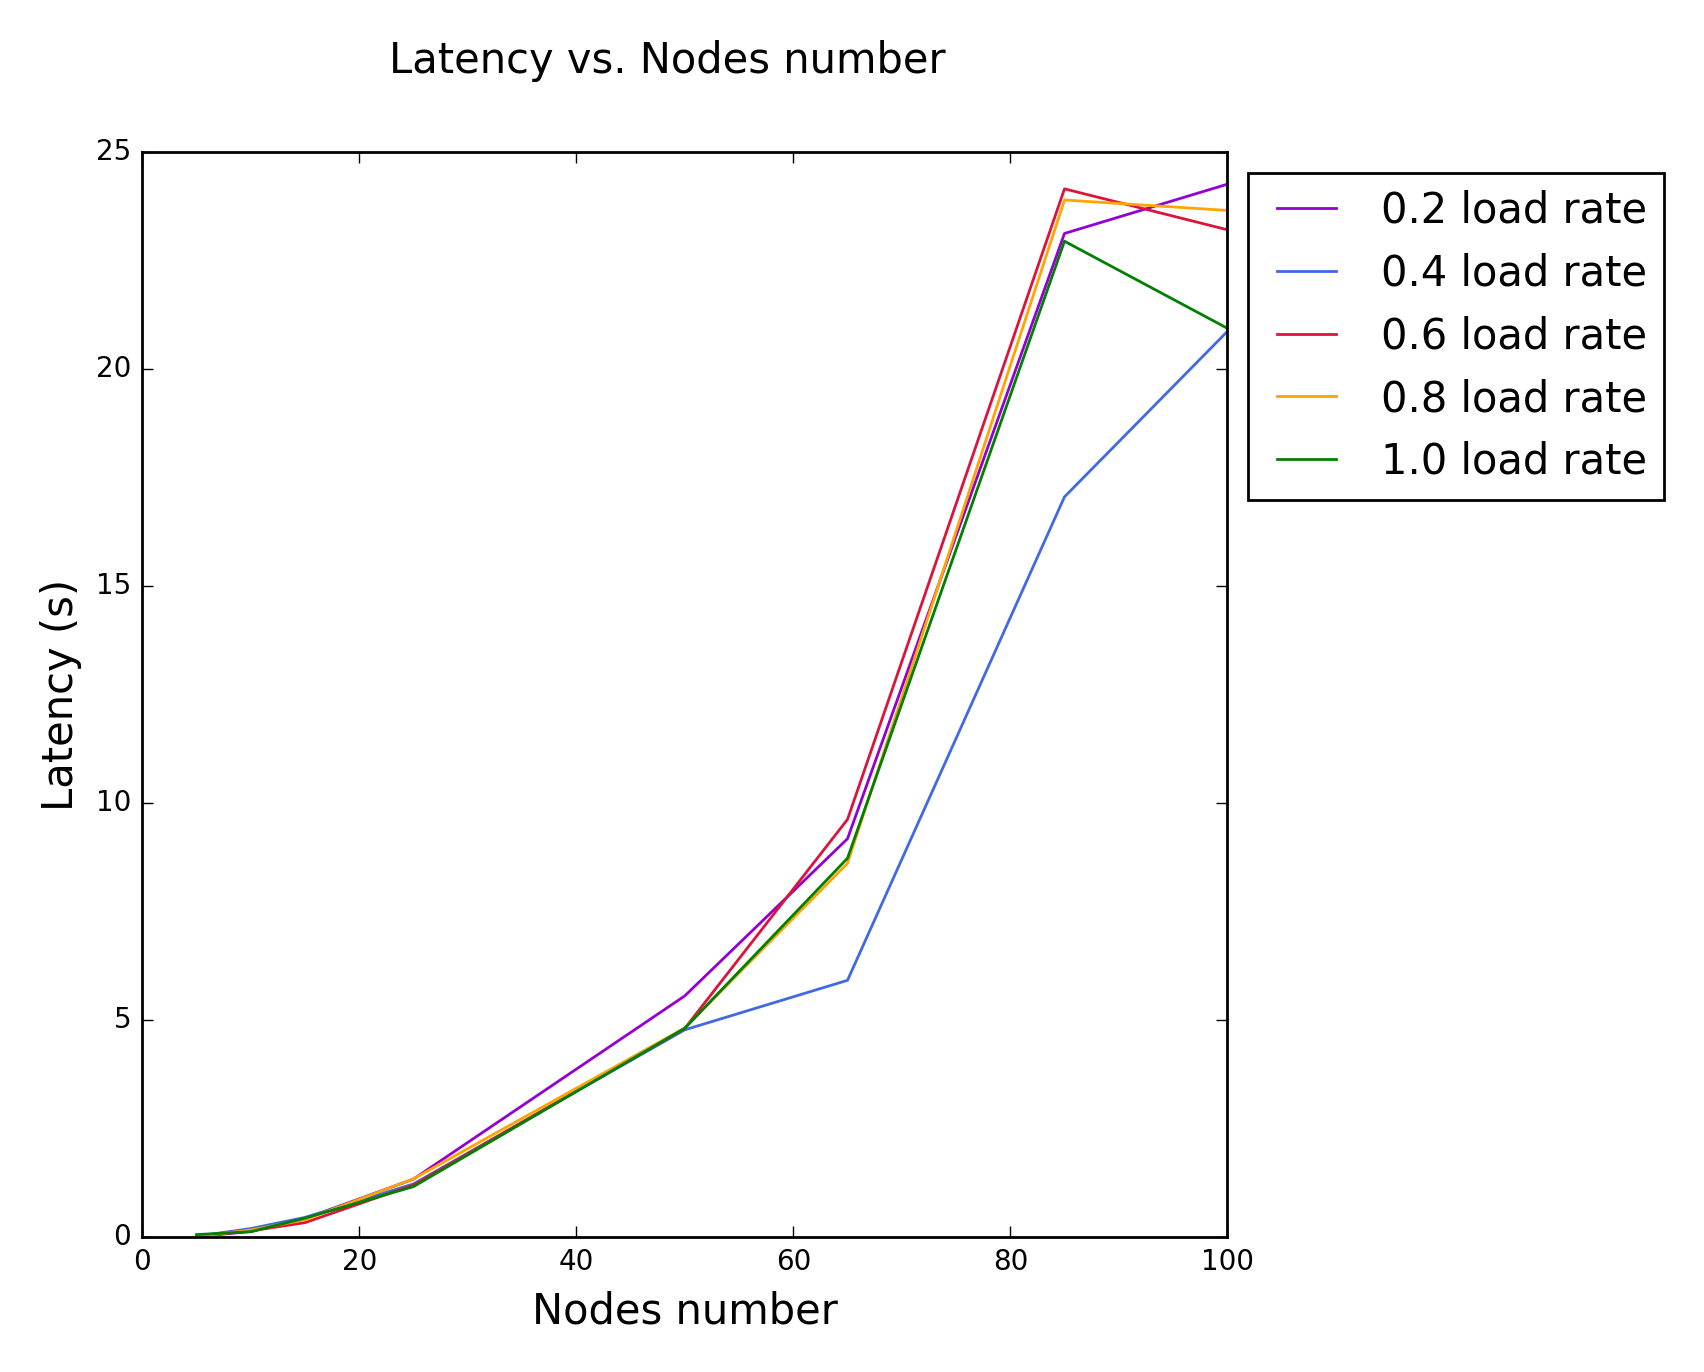
\includegraphics[width=0.7\textwidth]{Plots/LNN.png}
\caption{Зависимость latency от числа нод N}
\end{figure}

\begin{figure}[H]
\centering
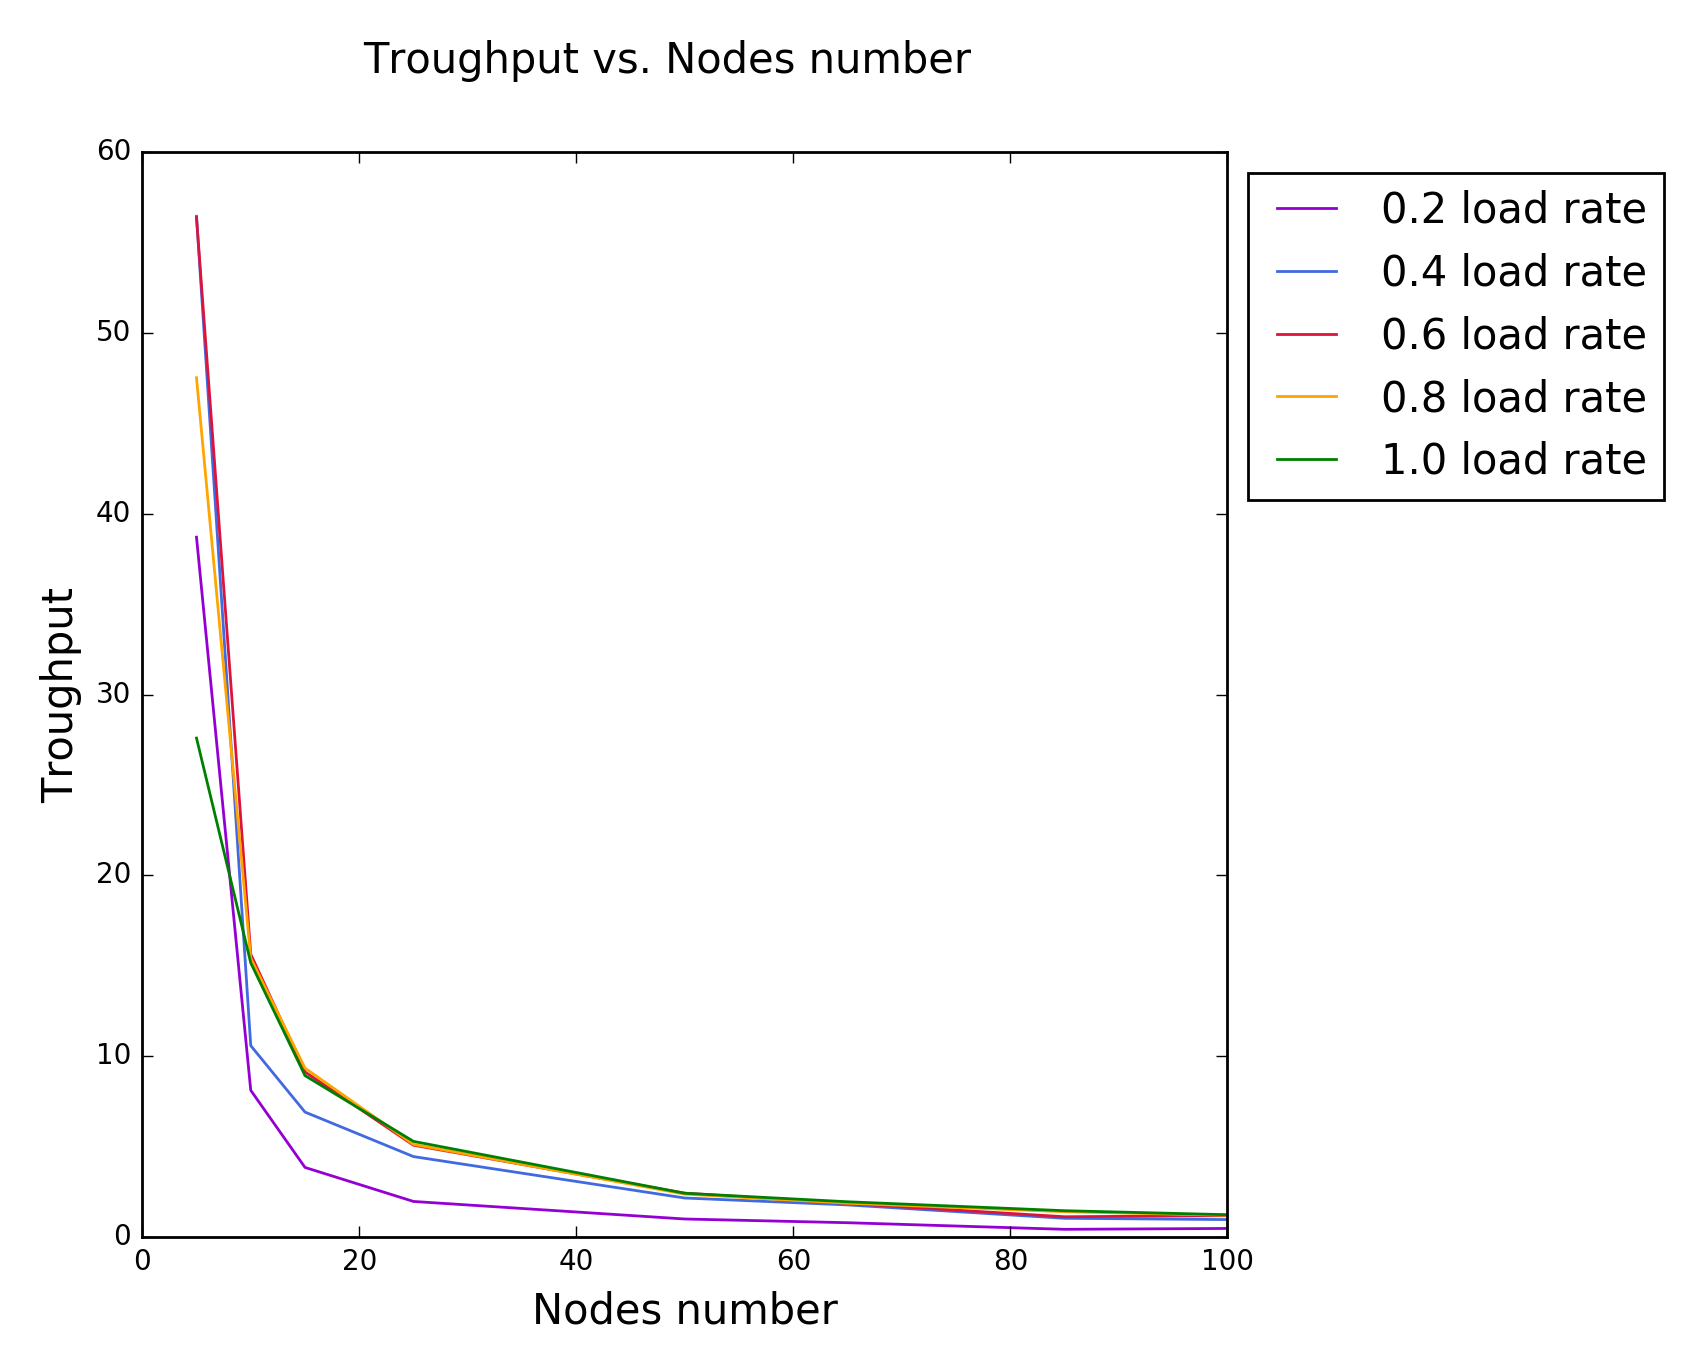
\includegraphics[width=0.7\textwidth]{Plots/TNN.png}
\caption{Зависимость throughput от числа нод N}
\end{figure}

\begin{figure}[H]
\centering
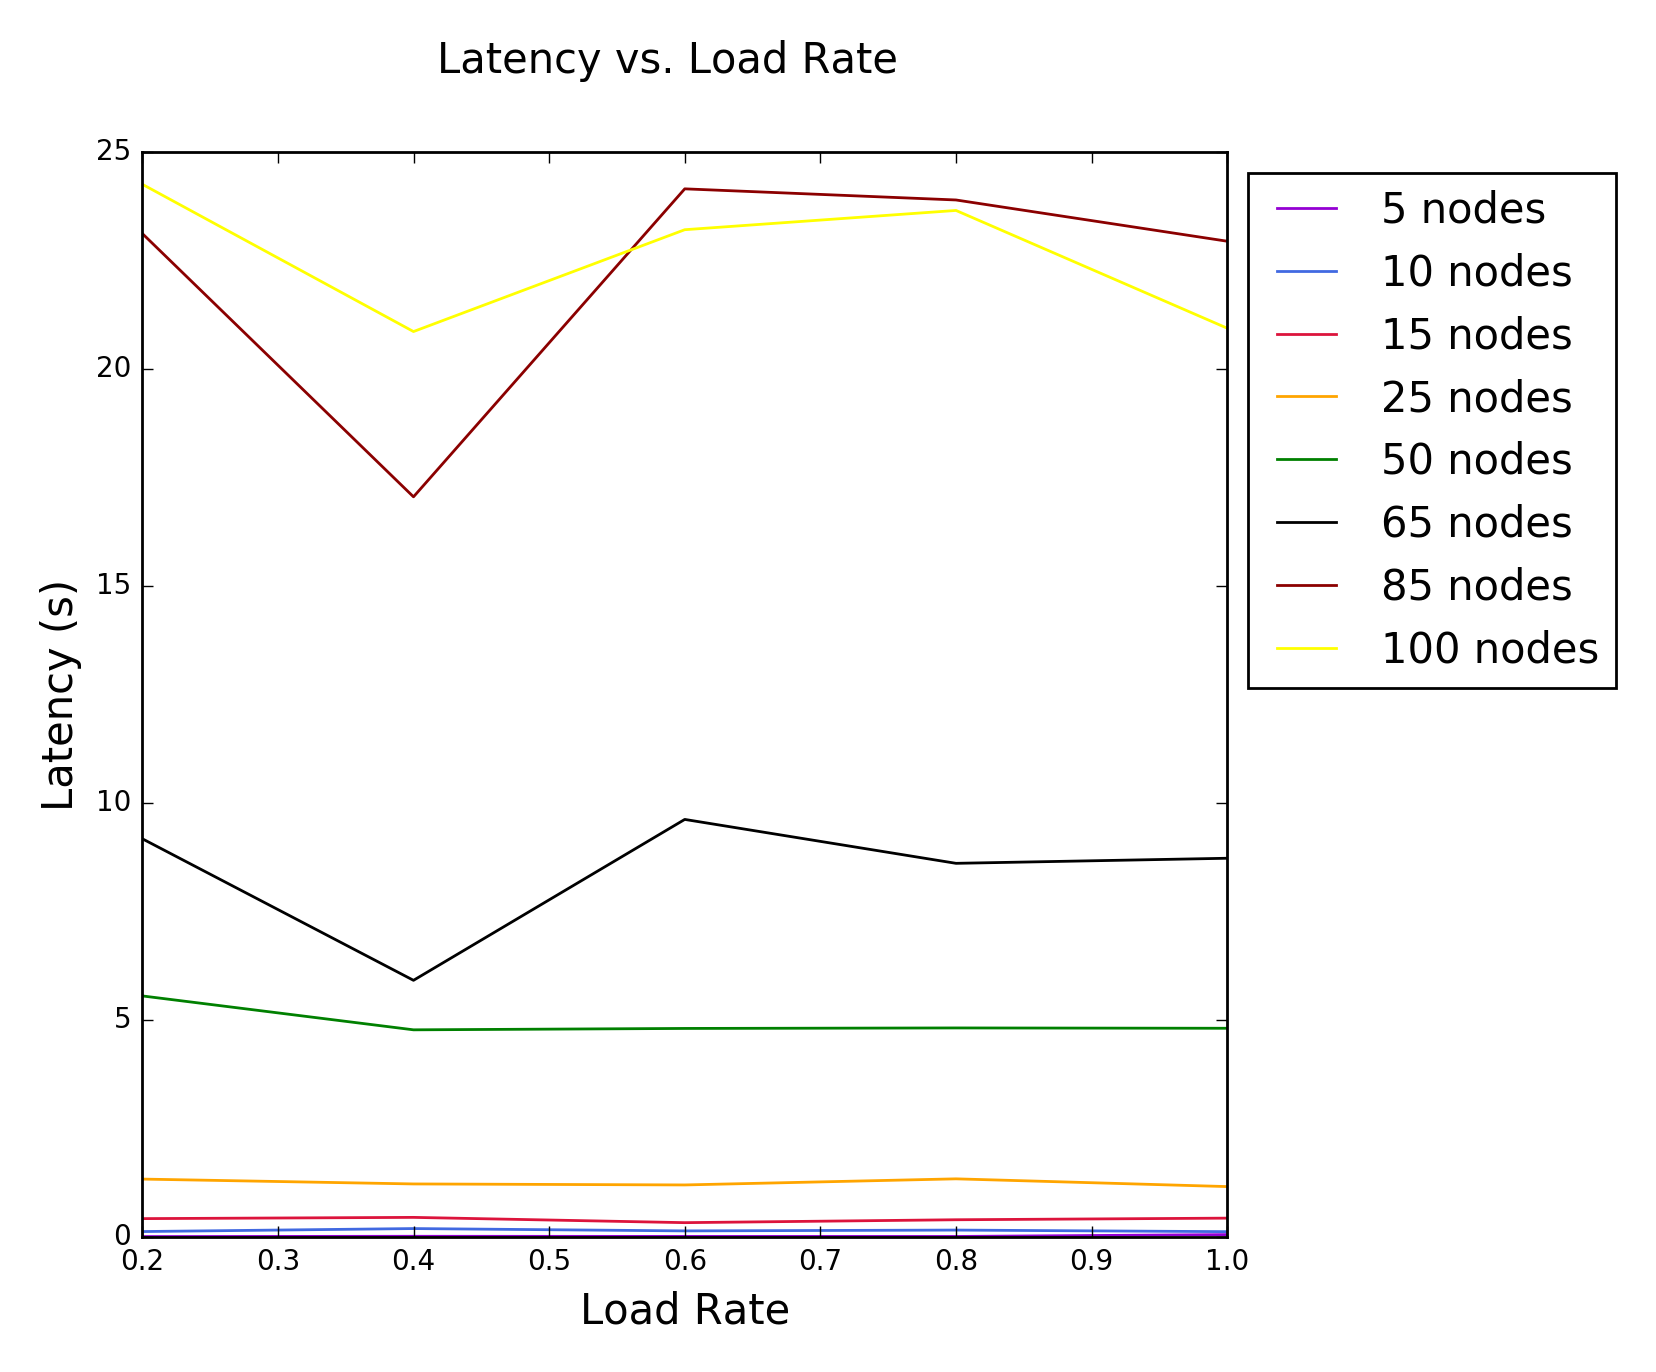
\includegraphics[width=0.7\textwidth]{Plots/LLR.png}
\caption{Зависимость latency от загрузки LR}
\end{figure}

\begin{figure}[H]
\centering
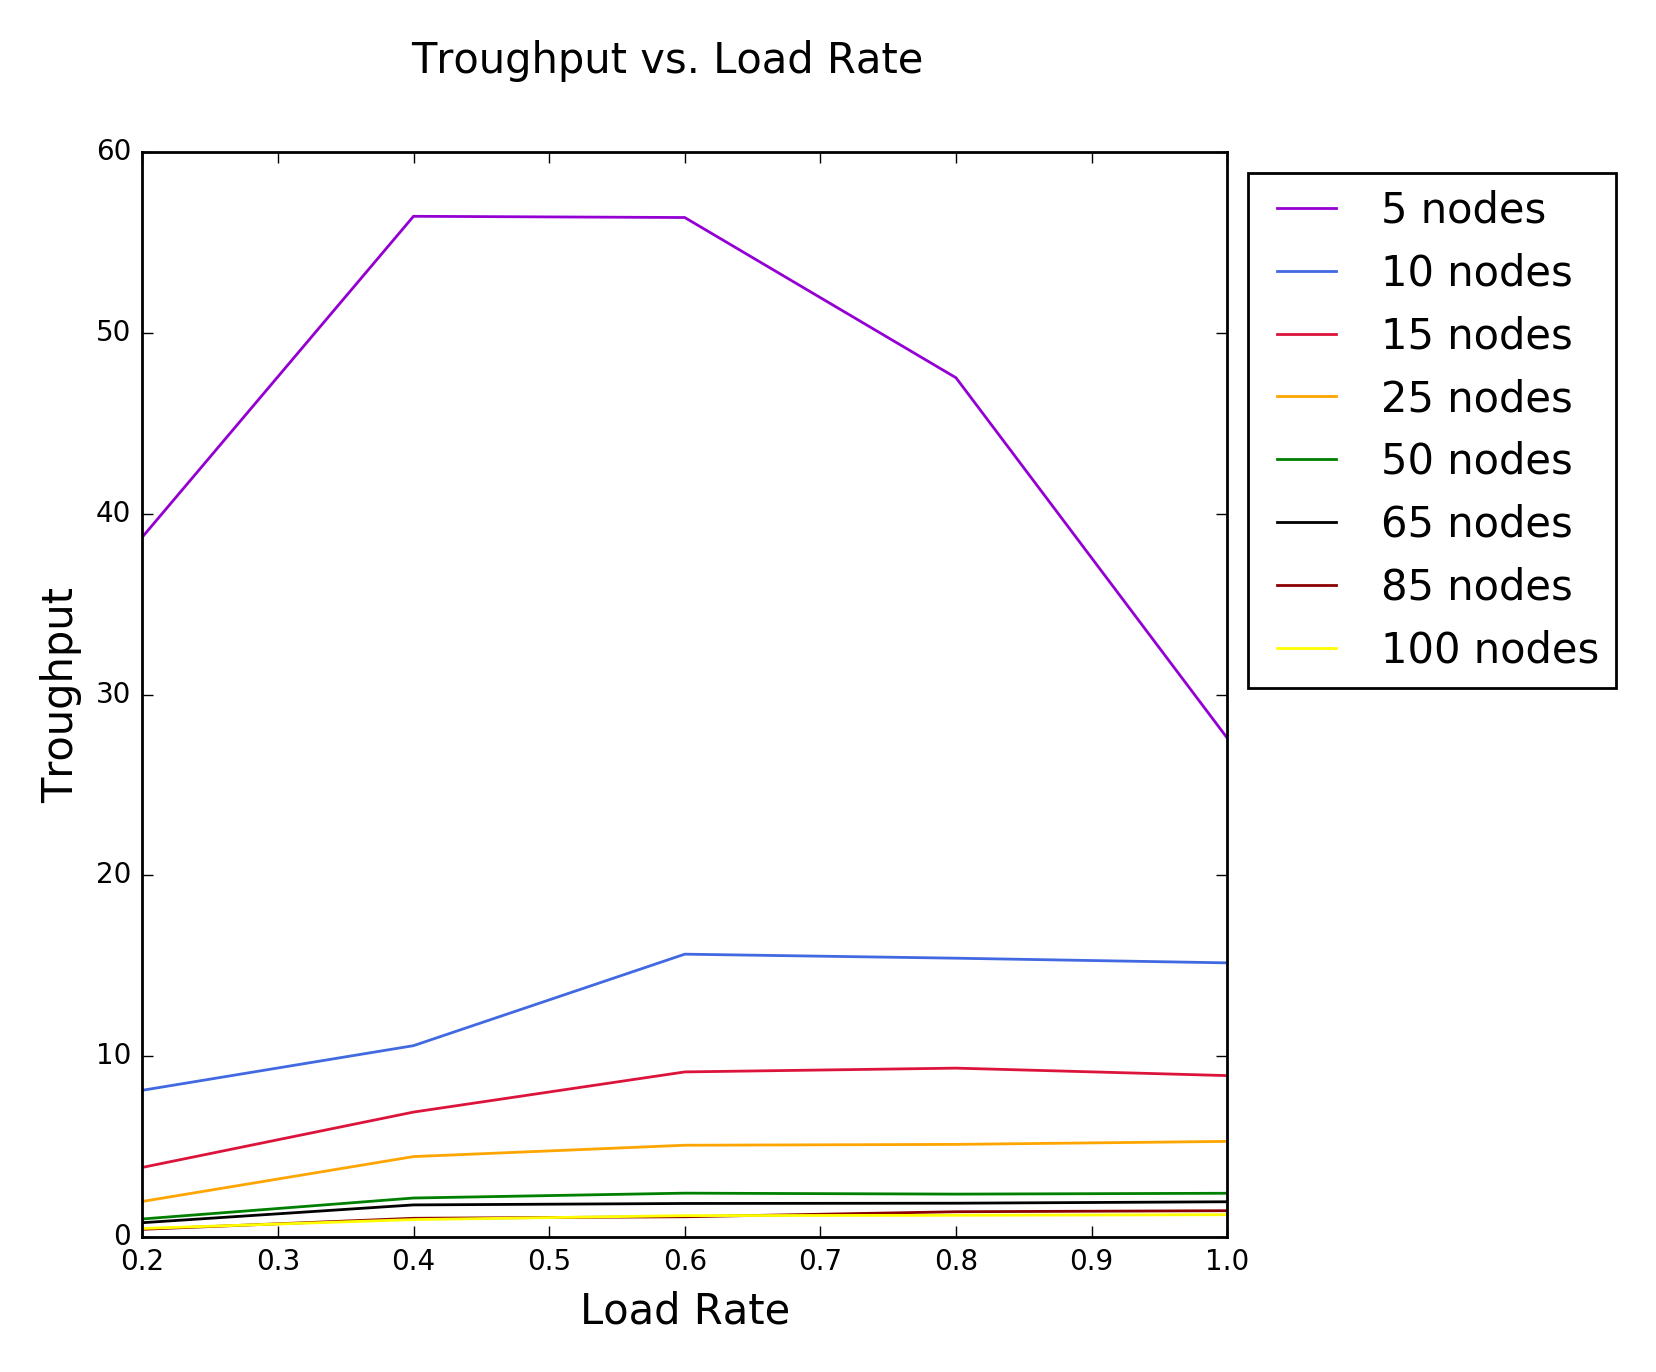
\includegraphics[width=0.7\textwidth]{Plots/TLR.png}
\caption{Зависимость throughput от загрузки LR}
\end{figure}

\subsection{Выводы}
В соответствии с результатами, на процессоре с двумя ядрами выгоднее использовать меньшее число узлов и с точки зрения latency, и с точки зрения throughput.

Для большого числа нод (65, 85, 100) с точки зрения latency выгоднее одновременно пересылать $0.4 * N$ сообщений.

Для $N = 5$ число пересылаемых сообщений $0.4 * N$ также оказывается выгодным с точки зрения throughput. 

\section{Исследование зависимости latency и throughput от token holding time при различных значениях загруженности ноды}

\subsection{Параметры}
Вероятность успеха доставки сообщения $p=0.75$.

Число нод $N = 15$.

Число фреймов принимало значения от 1 до 4 (недогруженный режим) и от 12 до 15 (перегруженный режим), т.е. $LR$ принимало значения \lstinline|{0.067, 0.133, 0.2, 0.267}| и \lstinline|{0.8, 0.867, 0.933, 1}|.

THT (token holding time) определялось следующим образом. Сначала  для определения l – среднего времени доставки сообщений – при выбранных $N$ и $LR$ производился калибровочный запуск с THT = \lstinline|Double.MAX_VALUE| (без ограничения сверху на время доставки сообщения). Затем THT определялся следующим образом: $l$ умножался на множитель из перечня: \lstinline|{0.7, 1.0, 1.5, 5.0, 10, 15, 20}|, который указан на графиках.
\newpage
\subsection{Результаты}

\begin{figure}[H]
\centering
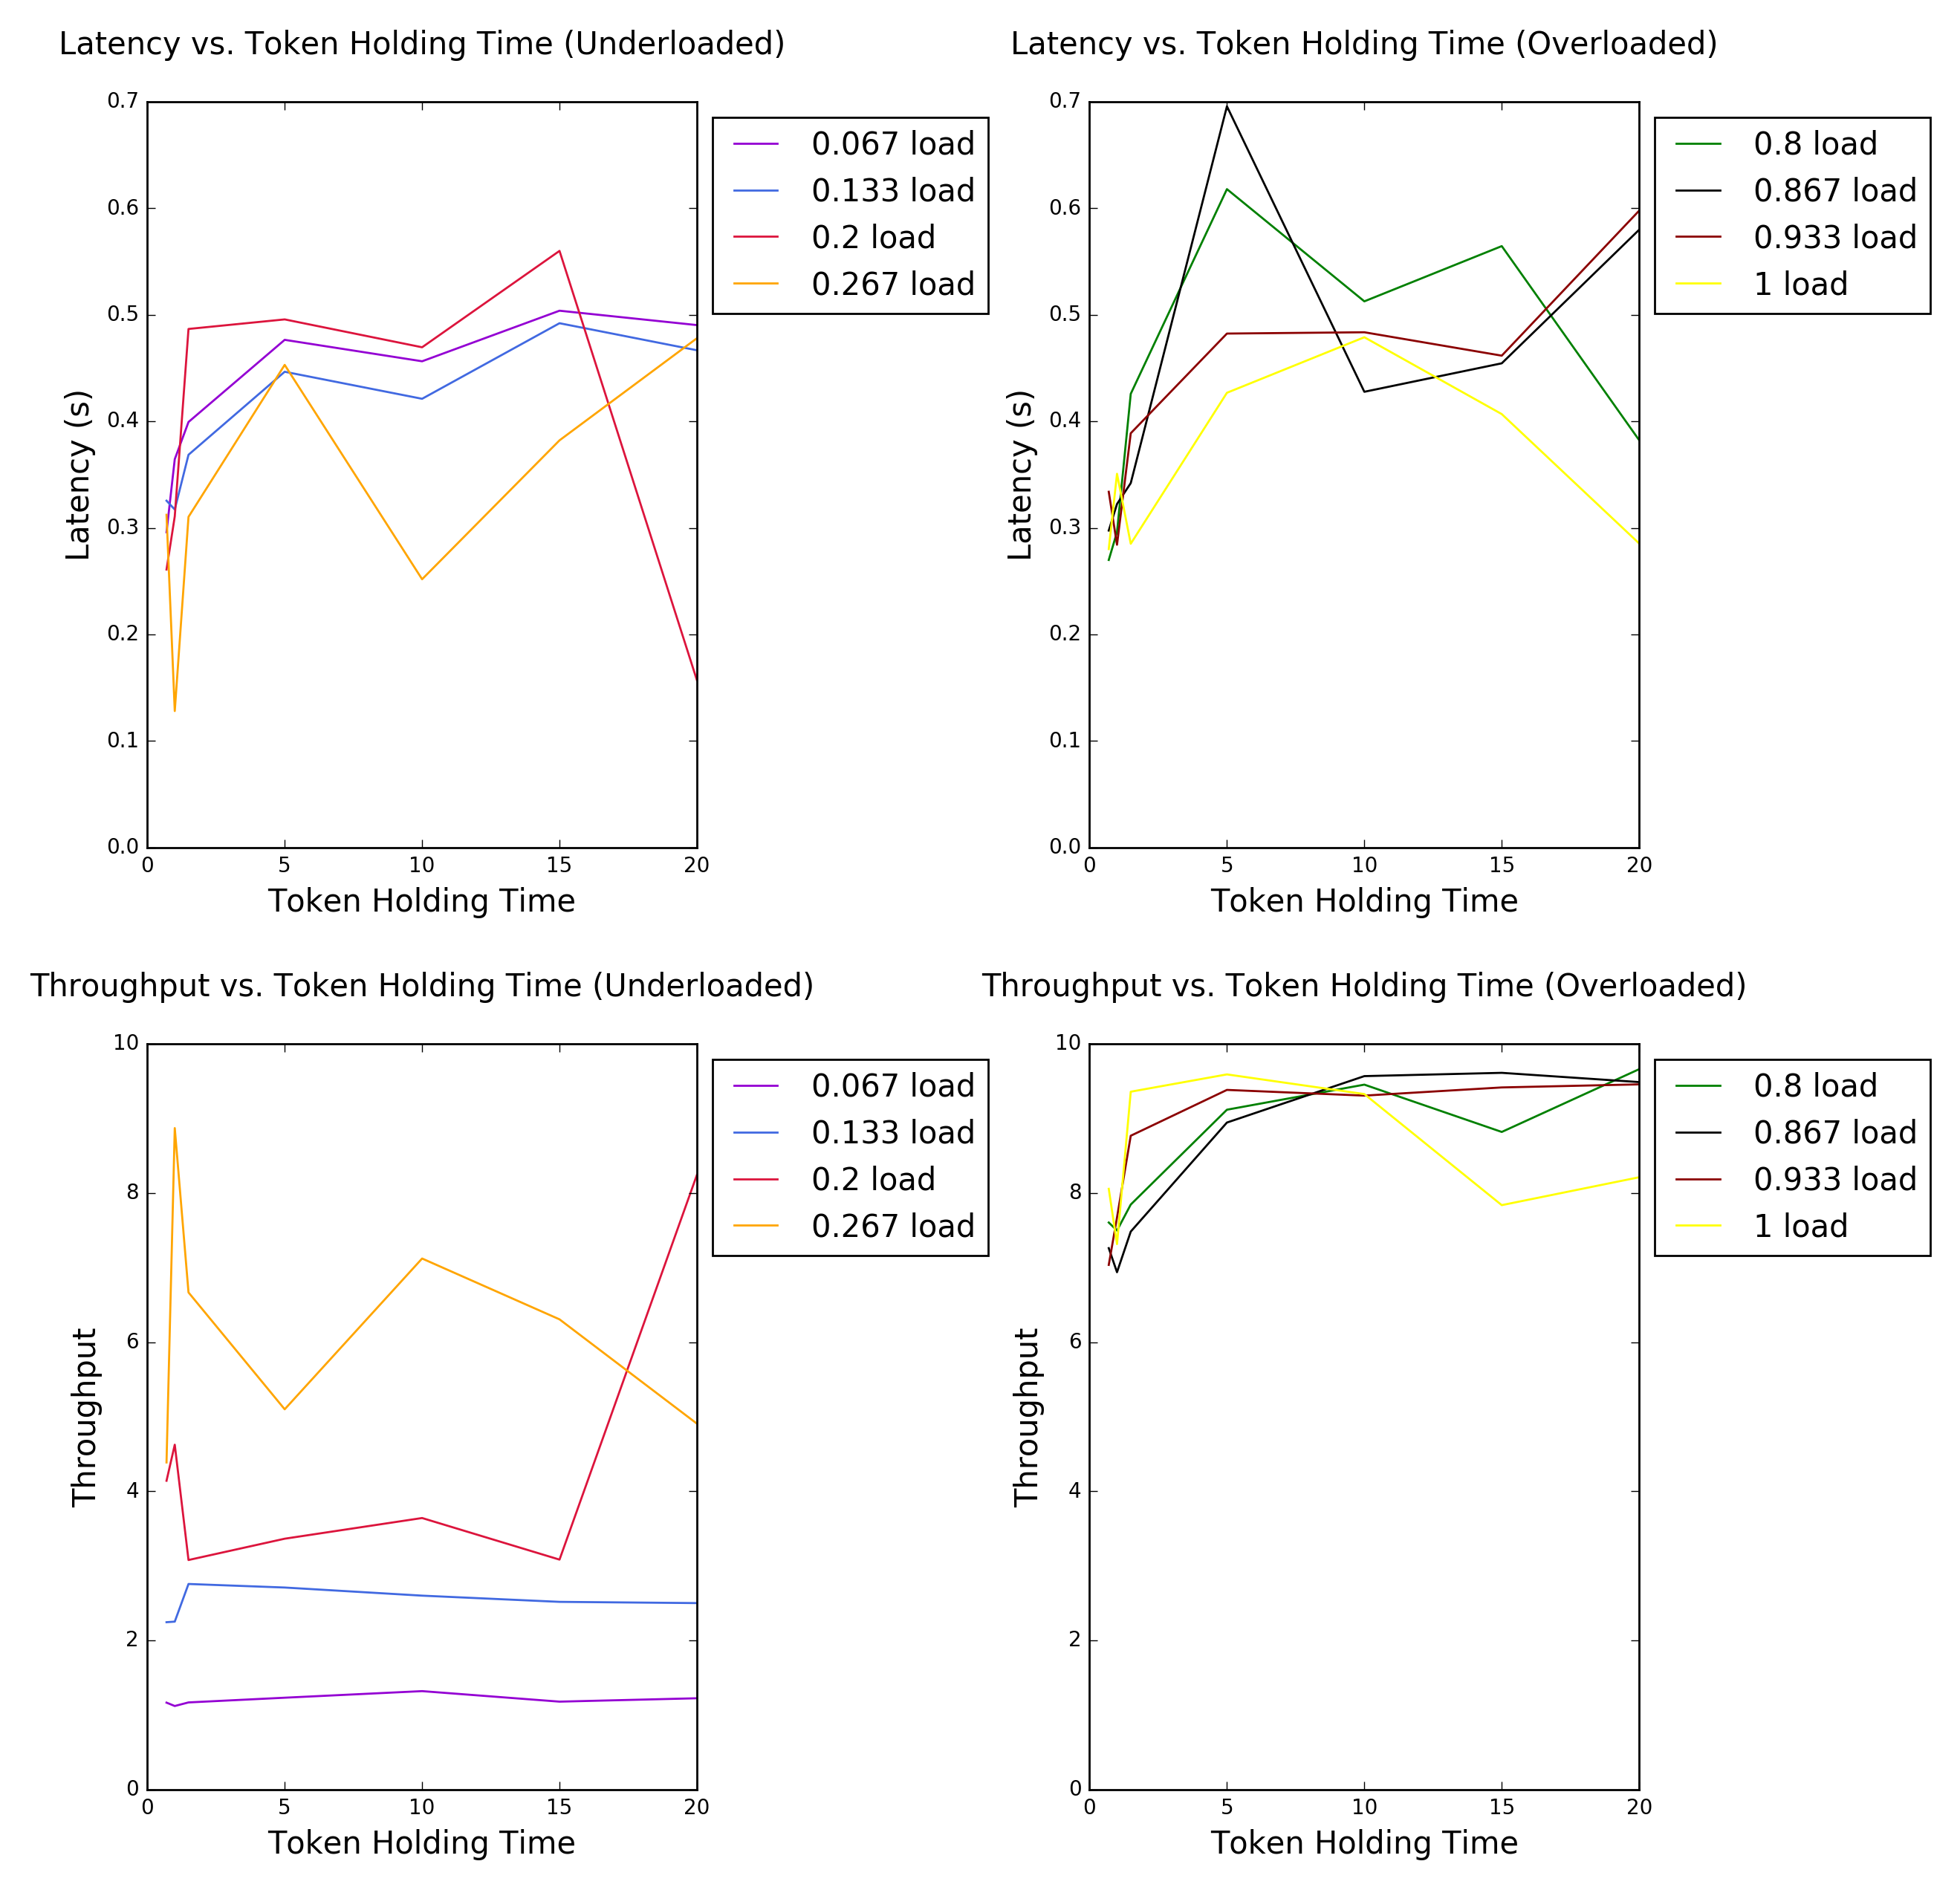
\includegraphics[width=1.1\textwidth]{Plots/THT.png}
\caption{Latency and Throughput vs. THT (Underloaded and Overloaded case)}
\end{figure}

\newpage
\subsection{Выводы}
Для недогруженного режима, скорее всего, будет выгодно взять множитель при l, описанный в разделе "Основные параметры и метрики", равным 0 (совершенно запретить повторные отправки).

Для перегруженного режима увеличение множителя даёт улучшение throughput, но ухудшение latency.

\addcontentsline{toc}{section}{Ссылки}
\renewcommand{\refname}{Ссылки} 
\begin{thebibliography}{9}
      \bibitem{o}
	  \url{http://web.chandra.ac.th/rawin/03-TokenRing.pdf}
	  
      \bibitem{w}
	  \url{https://en.wikipedia.org/wiki/Token_ring}

	  \bibitem{k}
	  \url{http://searchnetworking.techtarget.com/definition/Token-Ring}
	  
	  \bibitem{r}
	  \url{http://protocols.netlab.uky.edu/~calvert/classes/571/lectureslides/TokenRing.pdf}
\end{thebibliography} 


% \input Classes/Message

% \input Classes/Frame

% \input Classes/Node

% \input Classes/MessageGenerator

% \input Classes/Launcher

% \input Classes/LauncherExtract







\end{document}
